
\chapter{Project Segmentation's representation}
This section establishes how the project has been segmented across these 6 months. For better representaion we showcase the Gantt scheme and the Critical Path Analysis (CPA). 

\section{Gannt Scheme}
Below we present the Gannt scheme according to the workpackages \ref{gannt project} (Section 4). As mentioned before the phases are never superposed and are built upon each other. This project starts by preparing the foreground by studying the needs and the resources available and by planning the upcoming taks.But most of the work is condenced in the last 4 months of the project where there's the migration process and the deployment where the steps are verified by multiple tests.

\begin{figure}[h]
    \centering
    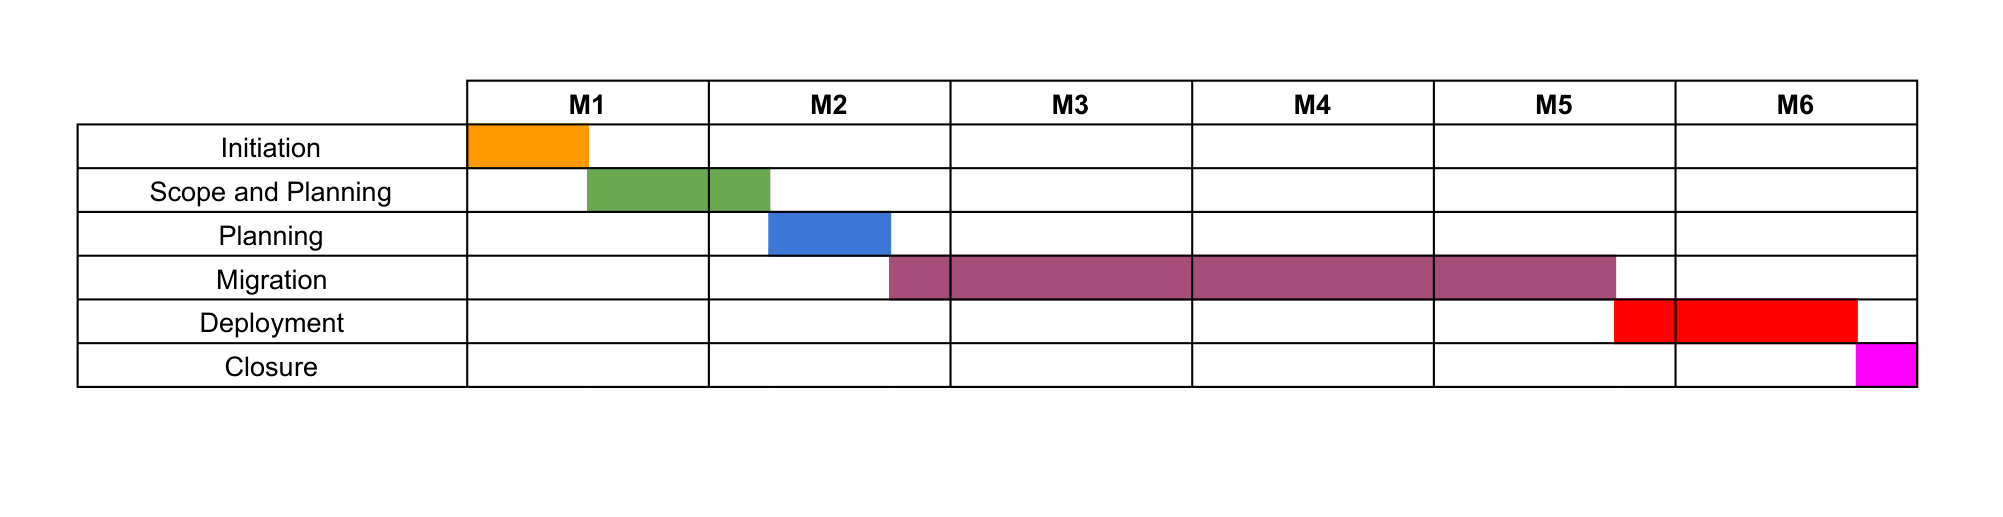
\includegraphics[width=\linewidth]{img/wp.png}
    \caption{Gannt Scheme for the full project}
    \label{gannt project}
\end{figure}

\subsection{Gannt Scheme for WP 1}
Below the detailed Gannt scheme for the first workpackage\ref{gannt wp1}. The last phase \textbf{"Charter Approval"} is essential to move to the next workpackage.  

\begin{figure}[h]
    \centering
    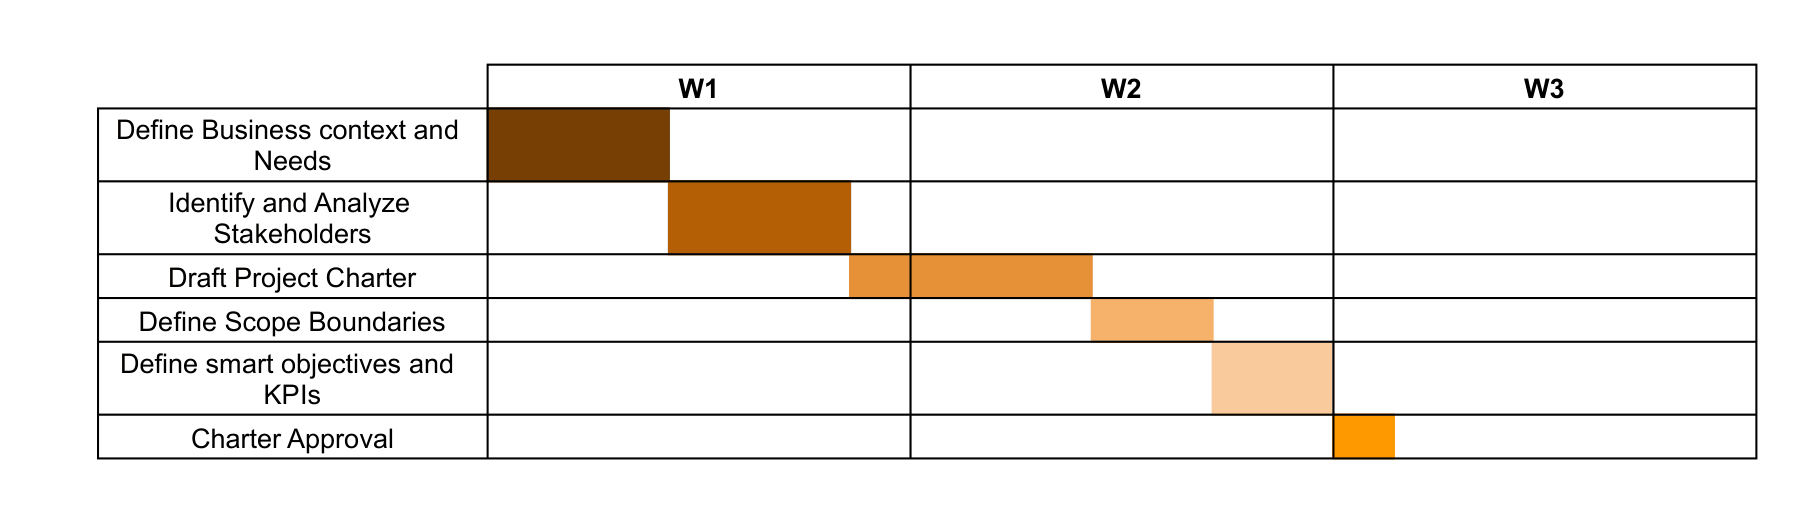
\includegraphics[width=\linewidth]{img/wp 1-1.png}
    \caption{Gannt scheme of the first workpackage: Initialtion}
    \label{gannt wp1}
\end{figure}

\subsection{Gannt Scheme for WP 2}
During this workpackage we defined the tasks that we have to tackle. A full \textbf{WBS dictionary} and the full\textbf{ requirements assessment} is expected to be able to move forward to the next workpackage. \ref{gannt wp2}

\begin{figure}[h!]
    \centering
    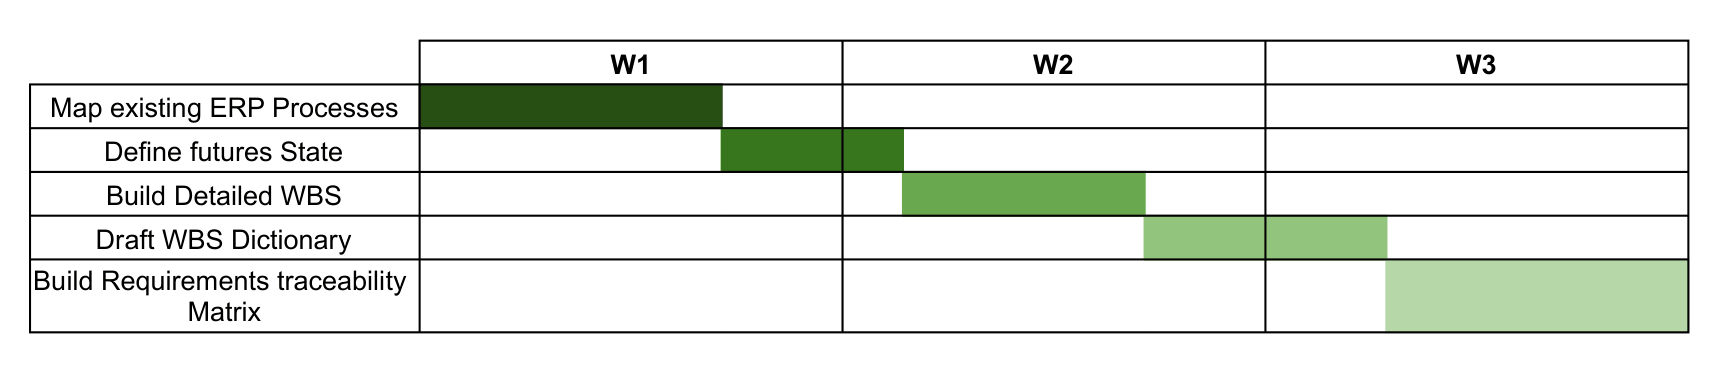
\includegraphics[width=\linewidth]{img/wp 2-1.png}
    \caption{Gannt scheme of the second workpackage: Scope and Planning}
    \label{gannt wp2}
\end{figure}

\subsection{Gannt Scheme for WP 3}
This is the last phase of the preparation and planning \ref{gannt wp3}. \textbf{the baseline approval} leads to the start of the main workpackage; the migration. 

\begin{figure}[h!]
    \centering
    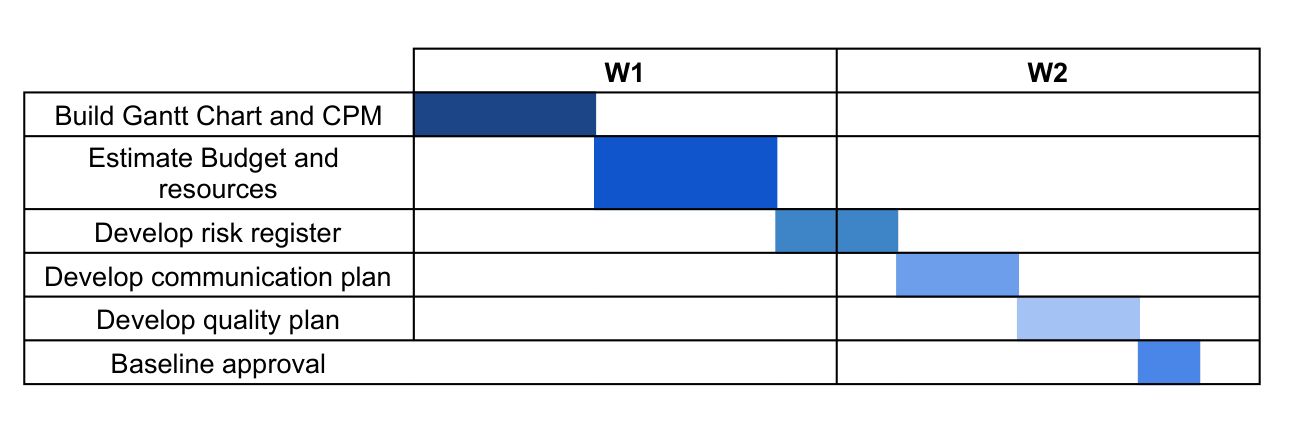
\includegraphics[width=\linewidth]{img/wp 3-1.png}
    \caption{Gannt scheme of the third workpackage: Planning}
    \label{gannt wp3}
\end{figure}

\subsection{Gannt Scheme for WP 4}
in the figure below\ref{gannt wp4} we represent the different phases of the main part of the project: the migration. As mentioned before this part takes the longest time as its different phases are more complex and time consuming. 
\textbf{Positive results obtained by testing the unit, the integration and by the users} is essential to move forward to the next workpackage. 

\begin{figure}[h!]
    \centering
    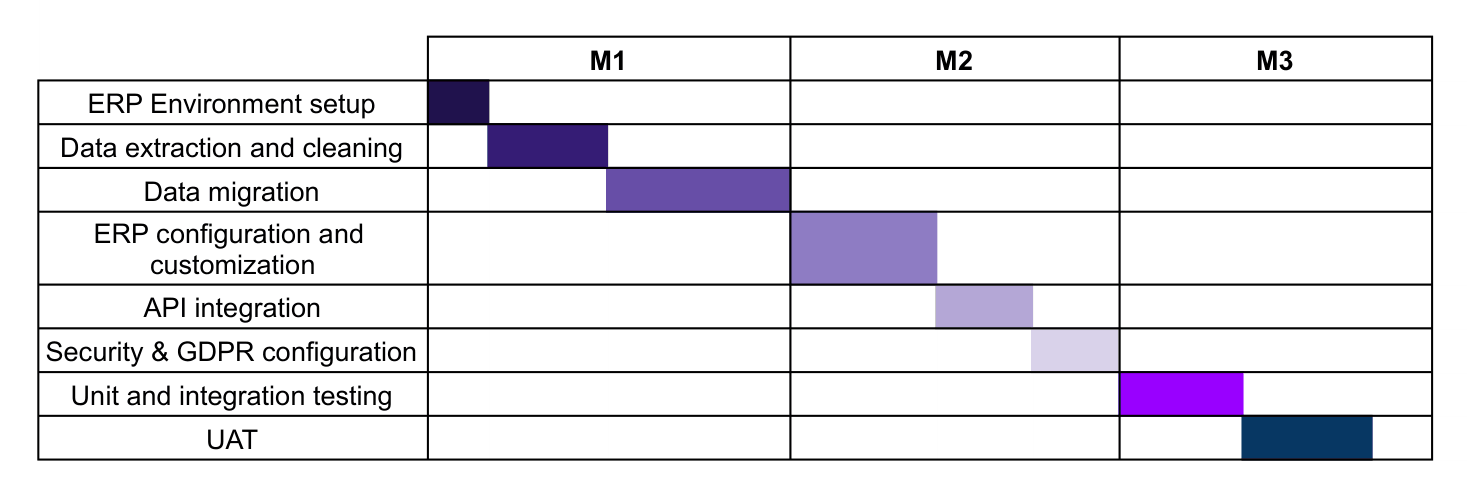
\includegraphics[width=\linewidth]{img/wp 4-1.png}
    \caption{Gannt scheme of the fourth workpackage: Migration}
    \label{gannt wp4}
\end{figure}

\subsection{Gannt Scheme for WP 5}
Once the tests were successful during the end of the last workpackage, the deployment can start as shown below\ref{gannt wp5}.  by the end of this workpackage \textbf{a full successful and fucntional migration should be put in plac}e. 

\begin{figure}[h!]
    \centering
    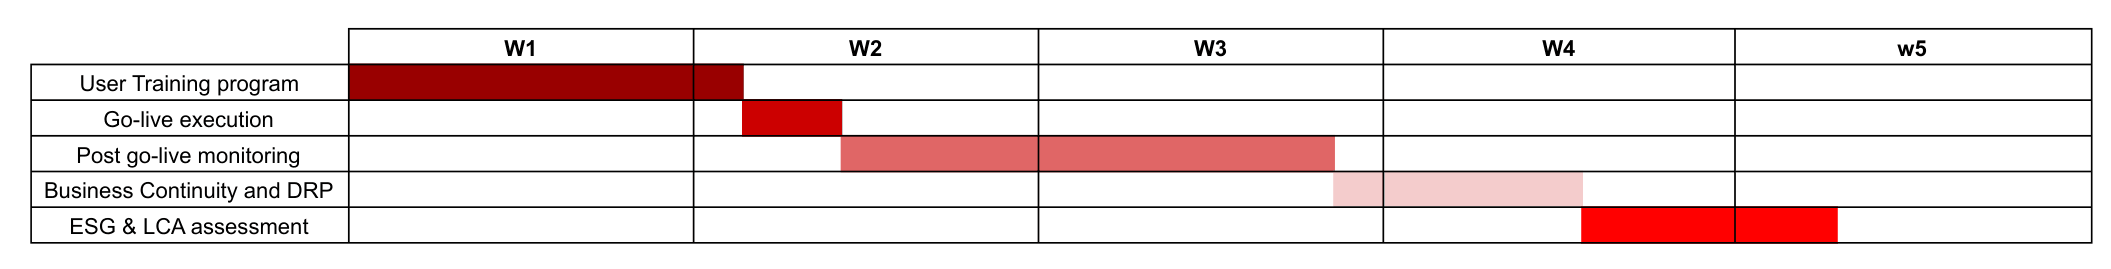
\includegraphics[width=\linewidth]{img/wp 5-1.png}
    \caption{Gannt scheme of the fifth workpackage: Deployment}
    \label{gannt wp5}
\end{figure}

\subsection{Gannt Scheme for WP 6}
After the successful deployment the closure can begin to end the project. This part is the shortest one. It's a step to assess the progress of the project and to review for future improvement and to avoid problems that were met during the execution of this one.\ref{gannt wp6}  

\begin{figure}[h!]
    \centering
    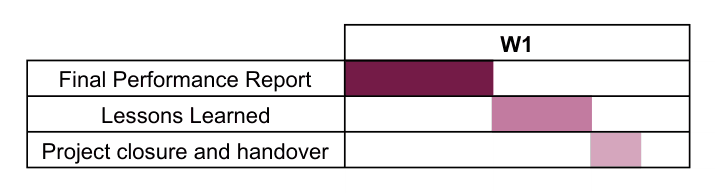
\includegraphics[width=0.5\linewidth]{img/wp 6-1.png}
    \caption{Gannt scheme of the sixth workpackage: Closure}
    \label{gannt wp6}
\end{figure}

\section{Critical Path Analysis (CPA)}
To better represent the dependencies between the different workpackages we represent the Critical Path Analysis shown below highlighting the requirements to move from a phase to another. 

\begin{figure}[h!]
    \centering
    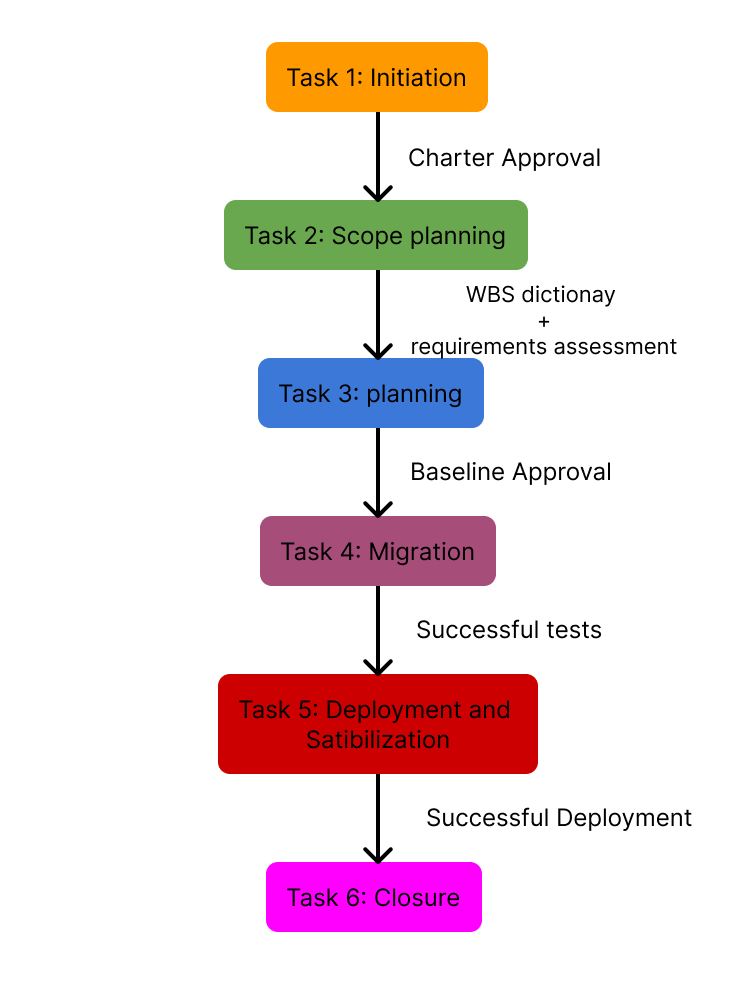
\includegraphics[width=0.5\linewidth]{img/pcm.png}
    \caption{CPA sheme for the full package}
    \label{gannt wp6}
\end{figure}


By applying these different schemes we ensured that every phase will take as much time as it demends and that no step was overlooked, thus it ensures the good development of the project and the balanced share of tasks.